 \documentclass[oneside,a4paper]{article}
\usepackage{ru-note}
\usepackage{indentfirst}
\hypersetup{
pdftitle={Теорема Александрова о вложении многогранников},
pdfauthor={Нина Лебедева и Антон Петрунин}
}


\begin{document}
%\pagestyle{empty}\renewcommand\includegraphics[2][{}]{}

\title{Теорема Александрова о\\ вложении многогранников}
\author{Нина Лебедева и Антон Петрунин}
\date{}
\maketitle

\begin{abstract}
Теорема Александрова даёт полное описание возможных внутренних метрик на поверхностях выпуклых многогранников.
Мы приводим набросок её доказательства.
\end{abstract}

\section{Введение}

Нас будет интересовать \emph{внутренняя метрика} на поверхности выпуклого многогранника;
то есть длина кратчайшей кривой на поверхности соединяющей две данные точки.
Напомним, что сумма углов при вершине многогранного выпуклого угла меньше $2\cdot \pi$; 
это утверждение можно найти в школьном учебнике А. П. Киселёва \cite[§~325]{kiselyov}.

Нетрудно видеть, что поверхность выпуклого многогранника гомеоморфна сфере.
Из вышесказанного получаем, что поверхность выпуклого многогранника наделённая естественной внутренней метрикой
является примером \emph{многогранной метрики на двумерной сфере с суммой углов вокруг каждой вершины не превосходящей $2\cdot\pi$}; 
метрика на сфере называется \emph{многогранной} если сфера допускает триангуляцию, 
такую что каждый её треугольник равен плоскому треугольнику.

Теорема Александрова гласит, что обратное верно если включить в рассмотрение многогранники вырождающиеся в плоские многоугольники.
В этом случае под его поверхностью понимается две копии многоугольника склеенные по границе
--- можно думать что многоугольник вырезан из картона и чтобы перейти с одной его стороны на другую сторону следует обогнуть периметр.

Везде далее мы предполагаем, что многогранник может вырождаться в плоский многоугольник.

\begin{thm}{Теорема Александрова}
\begin{enumerate}[I.]
\item\label{thm:exist} Многогранная метрика на сфере изометрична поверхности выпуклого многогранника тогда и только тогда, когда сумма углов при любой её вершине не превосходит $2\cdot\pi$.

\item\label{thm:unique} Более того, многогранник определяется метрикой на своей поверхности с точностью до конгруэнтности.
\end{enumerate}

\end{thm}

Две части этой теоремы называются теоремой существования и единственности.
(У Александрова имеется ещё и другая теорема единственности о многогранниках, обобщающая теорему Минковского).

Эта теорема играет ключевую роль в теории выпуклых поверхностей 
и несомненно она одна из самых удивительных теорем доказанных А.~Д. Александровым.
При этом её доказательство вполне элементарно, его можно объяснить любому, кто знакомом с азами топологии.

\begin{wrapfigure}{r}{\textwidth/2}
\vskip-0mm
\centering
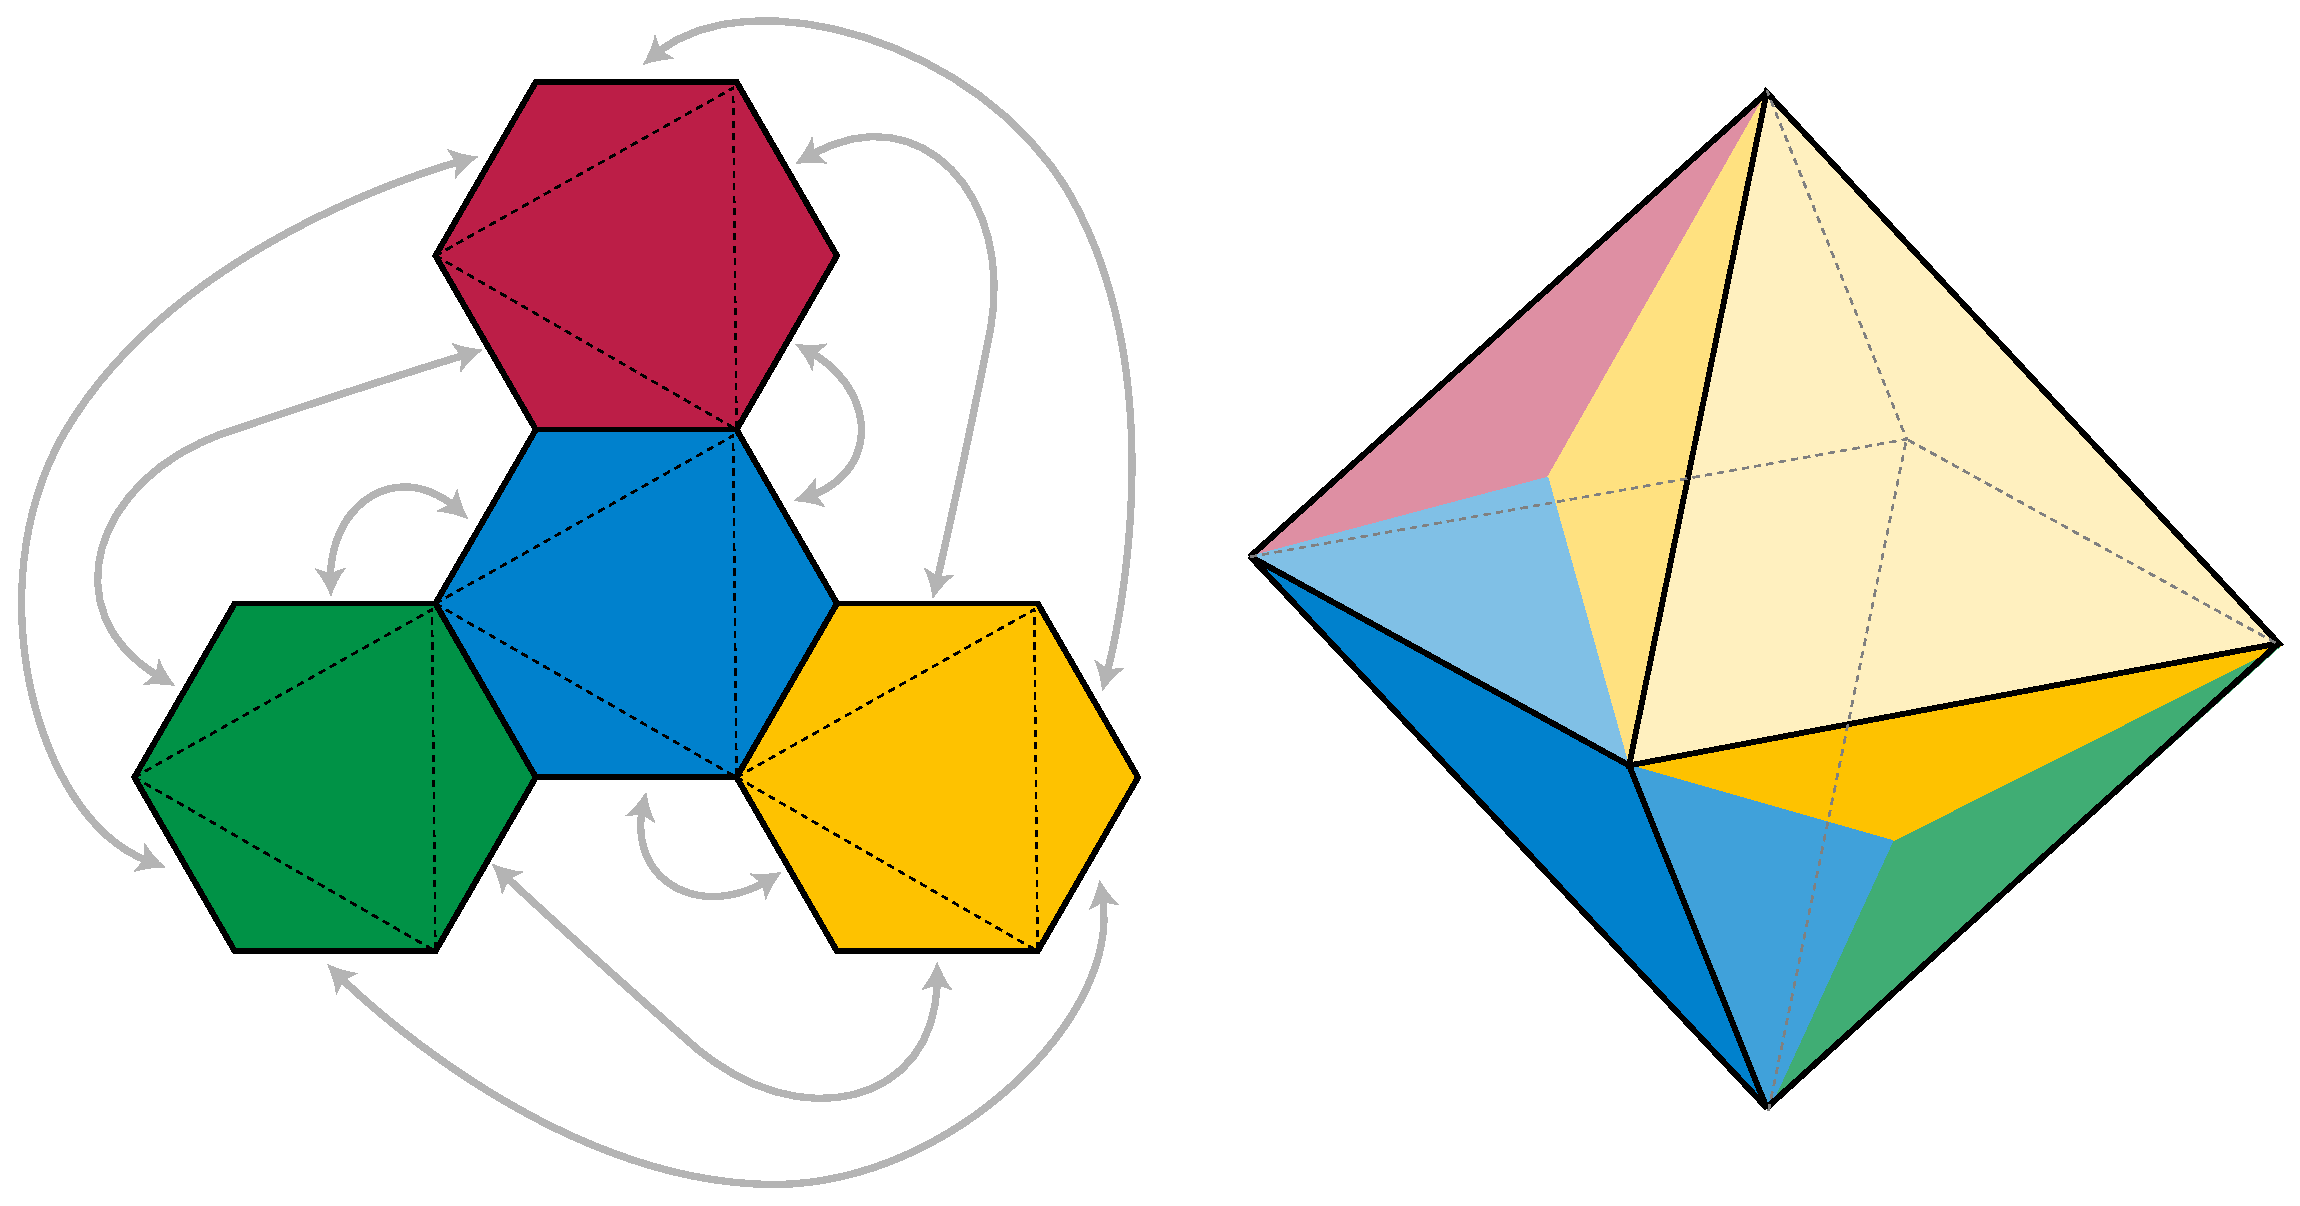
\includegraphics[width=\textwidth/2]{pics/4-hex_octahedron}
\vskip-0mm
\end{wrapfigure}

Согласно теореме, выпуклый многогранник полностью определяется внутренней метрикой своей поверхности.
Значит, зная метрику на поверхности можно в принципе узнать как пройдут рёбра многогранника.
Однако на деле это сделать непросто.
Например, поверхность склеенная из четырёх шестиугольников показанная слева есть поверхность октаэдра;
при этом линии склеек и некоторые вершины шестиугольников оказываются внутри граней октаэдра, и рёбра октаэдра вовсе не идут вдоль сторон шестиугольников.

Мы приведём набросок доказательства. 
Полное доказательство можно найти в замечательно написанной книжке самого Александра Даниловича~\cite{alexandrov}.


\section{Пространства многогранников и метрик}

\paragraph{Пространство многогранников.}
Обозначим через $\Phi$ пространство всех выпуклых многогранников в евклидовом пространстве, включая многогранники вырождающиеся в плоский многоугольник.
Многогранники в $\Phi$ будут рассматриваться с точностью до движения пространства сохраняющего ориентацию, а всё пространство $\Phi$ будет рассматриваться с естественной топологией (достаточно интуитивного понимания того, что два многогранника близки друг-другу).

Через $\Phi_n$ будем обозначать многогранники в $\Phi$ с ровно $n$ вершинами.
Поскольку любой многогранник в $\Phi$ имеет по крайней мере 3 вершины;
пространство $\Phi$ разбивается на счётное число подмножеств $\Phi_3,\Phi_4,\dots$

\paragraph{Пространство многогранных метрик.}
Пространство всех многогранных метрик на сфере с суммой углов вокруг каждой точки не более $2\cdot\pi$ будет обозначаться $\Psi$.
При этом метрики в $\Psi$ будут рассматриваться с точностью до изометрии сохраняющей ориентацию сферы, а всё пространство будет рассматриваться с естественной топологией (опять же, достаточно интуитивного понимания того, что две метрики близки).

Точка на сфере вокруг которой сумма углов строго меньше $2\cdot\pi$ будет называться \emph{существенной вершиной}.
Подмножество $\Psi$ состоящее из метрик с ровно $n$ существенными вершинами будет обозначаться $\Psi_n$.
Нетрудно видеть, что любая многогранная метрика в $\Psi$ имеет по крайней мере 3 существенных вершины;
и значит $\Psi$ разбивается на счётное число подмножеств $\Psi_3,\Psi_4,\dots$

\paragraph{От многогранника к его поверхности.}
Напомним, что поверхность выпуклого многогранника является многогранной метрикой на сфере с суммой углов вокруг каждой точки не более $2\cdot\pi$.
Заметим, что ориентация евклидова пространства определяет ориентацию поверхности многогранника.
Таким образом переход от многогранника к его поверхности определяет отображение 
\[\iota\:\Phi\to \Psi.\]

Заметим также, что число вершин многогранника равно числу существенных вершин его поверхности;
то есть вершин суммарный угол вокруг которых строго меньше $2\cdot\pi$.
Иначе говоря, $\iota(\Phi_n)\subset \Psi_n$ для любого $n\ge 3$.

\section{О доказательстве}

Используя обозначения, введённые в предыдущей секции, можно дать следующую более точную формулировку теоремы Александрова:

\begin{thm}{Переформулировка теоремы}
Для любого $n\ge 3$,
отображение $\iota$ является биекцией из $\Phi_n$ в $\Psi_n$.
\end{thm}

Приведённый ниже набросок основан на оригинальном доказательстве А. Д. Александрова.
Главное в нём это построение однопараметрического семейства многогранников, которое начинается с произвольного многогранника и заканчивается многогранником с поверхностью изометричной данной.  
Подобный ход рассуждений называется \emph{методом непрерывности};
он часто используются в теории дифференциальных уравнений.

\medskip

Две части теоремы доказываются отдельно.

\parit{Часть \ref{thm:unique}.} Докажем, что отображение $\iota\:\Phi_n\to\Psi_n$ инъетивно; иначе говоря многогранник определяется внутренней метрикой на своей поверхности с точностью до движения пространства сохраняющего ориентацию.

Последнее утверждение является уточнением теоремы Коши о многогранниках. 
Его доказательство практически повторяет доказательство Коши.

Теорема Коши утверждает, что грани многогранника вместе с правилом склейки полностью определяют выпуклый многогранник;
её доказательство приводится во многих классических популярных текстах \cite{aigner-zigler,dolbilin,tabacnikov-fuks}.

\medskip

\parit{Часть \ref{thm:exist}.} Докажем, что отображение $\iota\:\Phi_n\to\Psi_n$ сюрьетивно.
Это главная часть доказательства; она разбивается следующие леммы:

\begin{thm}{Лемма}
Пространство $\Psi_n$ связно.
\end{thm}

Доказательство этой леммы несложное, но требует изобретательности; 
его можно провести явным построением непрерывного однопараметрического семейства  метрик в $\Psi_n$ соединяющее две данных метрики.
Такое семейство можно получить путём последовательного применения следующего построения и ему обратного.

Пусть $M$ --- сфера с метрикой из $\Psi_n$, а $v$ и $w$ --- две существенные вершины в $M$.
Разрежем $M$ вдоль кратчайшей линии соединяющей $v$ и $w$. 
Заметим, что кратчайшая не проходит через другие существенные вершины в $M$.
Далее заметим, что существует трёхпараметрическое семейство заплаток, которыми можно заклеить разрез так, чтобы полученная метрика останется в $\Psi_n$; 
в частности, полученная метрика всё ещё будет иметь ровно $n$ существенных вершин (при этом вершины $v$ и $w$ могут перестать быть существенными).


\begin{thm}{Лемма}
Отображение $\iota\:\Phi_n\to\Psi_n$ открыто, 
то есть образ открытого множества в $\Phi_n$ открыт в $\Psi_n$.

В частности, для любого $n\ge 3$, множество $\iota(\Phi_n)$ открыто в~$\Psi_n$.
\end{thm}

Это утверждение очень близко к так называемой \emph{теореме об инвариантности области};
она утверждает, что непрерывное инъективное отображение между многообразиями равной размерности переводит открытые множества в открытые.
Доказательство этой теоремы проходит и в нашем случае так как оба пространства имеют размерность $3\cdot n-6$ и оба похожи на многообразия, хотя, формально говоря, таковыми не являются.

Мы ограничимся тем, что убедимся в том что размерность обоих пространств равна $3\cdot n-6$.

Выберем многогранник $P$ в $\Phi_n$.
Заметим, что $P$ однозначно определяется $3\cdot n$ координатами своих $n$ вершин.
При этом мы можем считать, что первая вершина совпадает с началом координат, у второй две координаты нулевые, а у третьей одна координата ноль; таким образом, для описания многогранников близких к $P$ достаточно $3\cdot n-6$ координат.
При этом, если многогранник не имеет симметрий, это описание можно сделать локально взаимно-однозначным;
в этом случае окрестность $P$ в $\Phi_n$ является $(3\cdot n-6)$-мерным многообразием.
При наличии у $P$ группы симметрий $\Gamma$ сохраняющей ориентацию, следует по ней профакторизовать;
так как группа конечна, размерность фактора останется той же.

Случай многогранных метрик аналогичен.
Необходимо построить разбиение сферы на плоские треугольники используя только существенные вершины.
По формуле Эйлера, получаем, что число рёбер в данном разбиении равно $3\cdot n-6$.
При этом длины рёбер однозначно определяют метрику, и небольшое изменение длин рёбер даёт метрику с теми же свойствами.


\begin{thm}{Лемма}
Отображение $\iota\:\Phi_n\to\Psi_n$ замкнуто, 
то есть образ замкнутого множества в $\Phi_n$ замкнут в $\Psi_n$.

В частности, для любого $n\ge 3$, множество $\iota(\Phi_n)$ замкнуто в~$\Psi_n$.
\end{thm}

Выберем замкнутое множество $Z$ в $\Phi_n$.
Обозначим через $\bar Z$ замыкание $Z$ в $\Phi$; заметим, что $Z=\Phi_n\cap \bar Z$.
Предположим $P_1,P_2,\dots\in Z$ --- последовательность многогранников, сходящихся к многограннику $P_\infty\in\bar Z$.
Заметим, что $\iota(P_n)$ сходится к $\iota(P_\infty)$  в $\Psi$.
В частности, $\iota(\bar Z)$ замкнуто в $\Psi$.

Поскольку $\iota(\Phi_n)\subset \Psi_n$ для любого $n\ge 3$ получаем, что  $\iota (Z)=\iota(\bar Z)\cap \Psi_n$, и лемма следует. 

\medskip

И так, $\iota(\Phi_n)$ --- непусто, замкнуто и открыто в $\Psi_n$, при этом $\Psi_n$ связно для любого $n\ge 3$.
Значит, $\iota(\Phi_n)=\Psi_n$; то есть, $\iota\:\Phi_n\z\to\Psi_n$ сюрьетивно.
\qeds

\sloppy
\printbibliography[heading=bibintoc]
\fussy

\end{document}
